% This must be in the first 5 lines to tell arXiv to use pdfLaTeX, which is strongly recommended.
\pdfoutput=1
% In particular, the hyperref package requires pdfLaTeX in order to break URLs across lines.

\documentclass[11pt]{article}

% Change "review" to "final" to generate the final (sometimes called camera-ready) version.
% Change to "preprint" to generate a non-anonymous version with page numbers.
\usepackage[review]{acl}

% Standard package includes
\usepackage{times}
\usepackage{latexsym}

% For proper rendering and hyphenation of words containing Latin characters (including in bib files)
\usepackage[T1]{fontenc}
% For Vietnamese characters
% \usepackage[T5]{fontenc}
% See https://www.latex-project.org/help/documentation/encguide.pdf for other character sets

% This assumes your files are encoded as UTF8
\usepackage[utf8]{inputenc}

% This is not strictly necessary, and may be commented out,
% but it will improve the layout of the manuscript,
% and will typically save some space.
\usepackage{microtype}

% Our packages
\usepackage{subcaption}
\usepackage{cleveref}
\usepackage{multirow}
\usepackage{multicol}
\usepackage{booktabs}
\usepackage{makecell}

\crefname{section}{Section}{Sections}%{\S}{\S\S}
% \crefname{table}{Tab.}{}
\crefname{table}{Table}{}
% \crefname{figure}{Fig.}{}
\crefname{figure}{Figure}{}
\crefname{section}{\S}{\S\S}
\Crefname{section}{\S}{\S\S}
\crefname{appendix}{Appendix}{Appendices}
\Crefname{Appendix}{Appendix}{}

% Our commands
\newcommand{\dieuwke}[1]{\textcolor{blue!70!black}{DH #1}}

% This is also not strictly necessary, and may be commented out.
% However, it will improve the aesthetics of text in
% the typewriter font.
\usepackage{inconsolata}

%Including images in your LaTeX document requires adding
%additional package(s)
\usepackage{graphicx}

% If the title and author information does not fit in the area allocated, uncomment the following
%
%\setlength\titlebox{<dim>}
%
% and set <dim> to something 5cm or larger.

\title{Lost in Inference: Rediscovering the Role of Natural Language Inference for Large Language Models}

% Author information can be set in various styles:
% For several authors from the same institution:
% \author{Author 1 \and ... \and Author n \\
%         Address line \\ ... \\ Address line}
% if the names do not fit well on one line use
%         Author 1 \\ {\bf Author 2} \\ ... \\ {\bf Author n} \\
% For authors from different institutions:
% \author{Author 1 \\ Address line \\  ... \\ Address line
%         \And  ... \And
%         Author n \\ Address line \\ ... \\ Address line}
% To start a separate ``row'' of authors use \AND, as in
% \author{Author 1 \\ Address line \\  ... \\ Address line
%         \AND
%         Author 2 \\ Address line \\ ... \\ Address line \And
%         Author 3 \\ Address line \\ ... \\ Address line}

\author{Lovish Madaan \\
  GenAI Meta, UCL \\
  \texttt{lovish@meta.com} \\\And
  David Esioubu \\
  GenAI Meta \\
  \texttt{esiobu@meta.com} \\\And
  Dieuwke Hupkes \\
  GenAI Meta \\
  \texttt{dieuwkehupkes@meta.com}}

%\author{
%  \textbf{First Author\textsuperscript{1}},
%  \textbf{Second Author\textsuperscript{1,2}},
%  \textbf{Third T. Author\textsuperscript{1}},
%  \textbf{Fourth Author\textsuperscript{1}},
%\\
%  \textbf{Fifth Author\textsuperscript{1,2}},
%  \textbf{Sixth Author\textsuperscript{1}},
%  \textbf{Seventh Author\textsuperscript{1}},
%  \textbf{Eighth Author \textsuperscript{1,2,3,4}},
%\\
%  \textbf{Ninth Author\textsuperscript{1}},
%  \textbf{Tenth Author\textsuperscript{1}},
%  \textbf{Eleventh E. Author\textsuperscript{1,2,3,4,5}},
%  \textbf{Twelfth Author\textsuperscript{1}},
%\\
%  \textbf{Thirteenth Author\textsuperscript{3}},
%  \textbf{Fourteenth F. Author\textsuperscript{2,4}},
%  \textbf{Fifteenth Author\textsuperscript{1}},
%  \textbf{Sixteenth Author\textsuperscript{1}},
%\\
%  \textbf{Seventeenth S. Author\textsuperscript{4,5}},
%  \textbf{Eighteenth Author\textsuperscript{3,4}},
%  \textbf{Nineteenth N. Author\textsuperscript{2,5}},
%  \textbf{Twentieth Author\textsuperscript{1}}
%\\
%\\
%  \textsuperscript{1}Affiliation 1,
%  \textsuperscript{2}Affiliation 2,
%  \textsuperscript{3}Affiliation 3,
%  \textsuperscript{4}Affiliation 4,
%  \textsuperscript{5}Affiliation 5
%\\
%  \small{
%    \textbf{Correspondence:} \href{mailto:email@domain}{email@domain}
%  }
%}

\begin{document}
\maketitle

\begin{abstract}
In the recent past, a popular way of evaluating natural language understanding (NLU), was to consider models' ability to do natural language inference (NLI) tasks. 
In this paper, we investigate if NLI tasks, that are rarely used for LLM evaluation, could also be still informative for evaluating LLMs.
Focussing on five different NLI benchmarks across six different models, we investigate if they are able to discriminate models of different size and quality and how their accuracies develop during training.
Furthermore, we investigate the extent to which the softmax distributions of models align with human distributions in cases where questions are ambiguous or vague.
Overall, our results paint a positive picture for the NLI tasks: we find that they are able to discriminate well between models at various stages of training, yet are not (all) saturated.
Furthermore, we find that while the distributional similarity with human label distributions improves with scale, it is still far above distributional similarity between two populations of humans, making it a potentially interesting statistic to consider in the future.
\end{abstract}


\section{Introduction}

Before the state-of-the-art (SOTA) in NLP was constituted almost exclusively by large language models (LLMs), a popular way of evaluating models' understanding of natural language was to consider their ability to perform \emph{natural language inference} (NLI) tasks \citep[most famously,][]{bowman-etal-2015-large,williams-etal-2018-broad}.
Motivated by the idea that concepts such as entailment and contradiction are central to many aspects of language meaning \citep{bowman-etal-2015-large}, in NLI tasks, a model is asked to judge the relationship between the meaning of two sentences, typically chosing between entailment, contradiction and no relationship.
% In this task, motivated by the idea that concepts such as entailment and contradiction are central to many aspects of language meaning \citep{bowman-etal-2015-large},  a model is asked to judge the relationship between the meaning of two sentences, typically chosing between entailment, contradiction and no relationship.
Included in the then widely-used natural language understanding benchmark GLUE \citep{wang2019glue}, the NLI benchmark \emph{Multi-Genre Natural Language Inference}  \citep[MNLI,][]{williams-etal-2018-broad} was up until relatively recently one of the most popular benchmarks to evaluate language models, and is -- with over 600 citations to date in 2024 -- well-cited even in the recent past.

However, with the arrival of LLMs, MNLI and other datasets have lost their spot on the SOTA leaderboards.
With the exception of \citet{brown2020language},  who reported low scores for GPT-3 on the NLI benchmark \emph{Adversarial NLI} \citep[ANLI,][]{nie-etal-2020-adversarial}, not a single LLM release paper considers an NLI benchmark in their evaluation suite.\footnote{However, some recent papers have reported low scores for GPT3.5 for XNLI \citep{ohmer2024form,ohmer-etal-2023-separating} and for Llama 1 models on ANLI, HANS \citep{mccoy-etal-2019-right} and MNLI \citep{weber-etal-2023-mind}.}
In this paper, we investigate why.
Are NLI benchmarks simply not suitable to evaluate modern-day LLMs? 
Are their examples too difficult or too easy?
Are their scores for some reason not informative?
Or do they, in fact, still provide a useful signal, but has the community simply forgotten about them?

Focussing on five different NLI benchmarks across six different models, we first investigate if they are able to discriminate models of different size and quality (\cref{subsec:fully_trained}), finding that they can, but that one or more shots are needed to obtain a somewhat reasonable accuracy for models of any size.
We furthermore show that performances on the datasets develop steadily during training, albeit with some fluctuations, making the benchmarks suitable for monitoring training progress (\cref{subsec:during_training}).
For some of the benchmarks, accuracies of the best models are touching 80 or even 90, for ANLI \citep{nie-etal-2020-adversarial}, however, the accuracy of even the best model does not exceed 70.
% \paragraph{Benchmarks} In our experiments, we consider five NLI benchmarks: ANLI \citep{nie-etal-2020-adversarial}, HansNLI \citep{mccoy-etal-2019-right}, MNLI \citep{williams-etal-2018-broad}, SNLI \citep{bowman-etal-2015-large}, and $\alpha$NLI \citep{bhagavatula2020abductive}. 
% Furthermore, we find next to no contamination of the benchmarks in common pretraining corpora.
Next, we investigate the extent to which improvement on the higher-scored benchmarks is still possible (\cref{subsec:saturation}).
In a manual analysis, we find that, for the best performing models, some examples with incorrect predictions are in fact incorrect, but most concern questions on which humans may disagree too.
Motivated by this result, we further explore this topic by considering the benchmark ChaosNLI \citep{nie-etal-2020-learn}, which contains 100 human annotations for over 4500 samples of three of the benchmarks we consider (\cref{subsec:chaosnli_dist}).
We find that accuracies (as computed on the majority label) are higher if the entropy of the human labels is low; when humans disagree, models are more likely to select one of the less preferred labels.

Finally, we consider the distributional differences between model outputs and human labels, as measured by the Jensen Shannon Divergence (JSD) between the human label distributions and the models' softmax distributions over the possible answers.
We find that the JSDs are lower (thus: better) than the ones reported by \citet{nie-etal-2020-learn} for the previous generation of models, and they are also better than chance distributions. 
However, they are still substantially higher than the JSD between two populations of humans, bearing interesting implications on the viablity of using an ensemble of LLM judges as a `jury' \citep[e.g.][]{verga2024replacing}.
Interestingly, contrary to the findings of \citet{nie-etal-2020-learn}, we do observe an effect of scale and model quality: JSD shows a clear and steady decrease during training, and larger models have lower JSD than smaller models.

In sum, we find that NLI benchmarks are still relevant for model development and improvement.
Specifically, they are able to discriminate between models of different scale and quality, develop steadily during training, and are not completely saturated.
Furthermore, as even the best models are still far away from humans in this respect, we see promise in monitoring the development of the distributional differences between models and humans, both during and at the end of training.



\section{Related work}

Before presenting our analysis, we first discuss NLI or \emph{recognising textual entailment} (RTE) tasks (\cref{related:nli}) and touch upon the related topic of subjectivity for NLP tasks (\cref{related:subjectivity}) before presenting our analysis.

\subsection{RTE tasks and their results}
\label{related:nli}

In RTE tasks -- also referred to as `natural language inference' (NLI) tasks, models are asked to judge whether the meaning of one sentence can be inferred from the meaning of another.
Because the concept of entailment (and contradiction) are considered central to many aspects of language meaning \citep[e.g.][]{bowman-etal-2015-large}, such tasks were for some period considered an important task to determine whether one model could understand language better than another \citep{poliak-2020-survey}.
Over the years, many different, increasingly more difficult NLI tasks have been proposed in the literature.
Included in the popular benchmarks GLUE \citep{wang2019glue} and SuperGLUE \citep{wang2019superglue}, the benchmarks MNLI \citep{williams-etal-2018-broad} and RTE \citep{dagan2005pascal} and RTE were used to claim SoTA by many influential models such as BERT \citep{devlin2019bert} and T5 \citep{raffel2023t5}.
When performance on MNLI and RTE started to saturate, several adversarial NLI benchmarks were introduced, such as ANLI \citep{raffel2023t5} and HANS \citep{mccoy-etal-2019-right}, on which BERT-style models performed poorly compared previous datasets.
For LLMs, NLI benchmarks are rarely used.
Of all big LLM releases, only GPT-3 \citep{brown2020language} reported an NLI score, and only on one partition of ANLI.
They concluded that NLI is a difficult task for general purpose LLMs.
Similar trends were observed by \citet{ohmer2024form} and \citet{weber-etal-2023-mind} for decoder-only LLMs on various NLI tasks, in part motivating the study presented here.

\subsection{Subjectivity in NLP tasks}
\label{related:subjectivity}
Another line of work relevant to ours considers the behaviour of models in cases where humans disagree on the correct label for a particular sample. 
The ground truth labels for benchmarks like MNLI and SNLI are decided according to the majority label by human annotators. 
This simplifies the data annotation process, while also making the evaluation easier by framing it as a classification task. 
However, previous studies \citep{pavlick-kwiatkowski-2019-inherent, nie-etal-2020-learn} showed that significant disagreement exists for a large number of these datasets because the meaning of a sentence can differ based on context and background knowledge, and the ground truth label according to a human annotator depends on their understanding of this context. 
These disagreements were captured in more detail in the dataset ChaosNLI \citep{nie-etal-2020-learn}, comprising of 100 annotations for each sample for a subset of three benchmarks -- MNLI, SNLI, and $\alpha$NLI.
As human disagreements are ubiquitous yet often ignored in evaluation, in our study, we analyse not only the model accuracies, but also the relationship between these disagreements and models' probability distributions across the different labels.
A study with a similar aim was presented by \citet{chen2024seeingbig}, who explored whether the softmax probability distributions of two LLMs across the labels in ChaosNLI and VariErr NLI \citep{weber-genzel-etal-2024-varierr} can approximate the Human Judgement Distribution (HJD) across the labels. 
\citet{baan-etal-2024-interpreting} further analysed how the softmax probability distribution can be interpreted both as an approximation to human label distribution and confidence estimation in language models.


\section{Setup}

\paragraph{Benchmarks} In our experiments, we consider five NLI benchmarks: ANLI \citep{nie-etal-2020-adversarial}, HANS \citep{mccoy-etal-2019-right}, MNLI \citep{williams-etal-2018-broad}, SNLI \citep{bowman-etal-2015-large}, and $\alpha$NLI \citep{bhagavatula2020abductive}. 
The number of examples and labels for each dataset are present in Table \ref{tab:dataset}. 
For MNLI and SNLI, we filter out the noisy test samples for which there is no ground truth available for the evaluation. % Dieuwke: not entirely clear to me what this means

\paragraph{Models} For each of these benchmarks, we compute and analyse scores for three different model families: Llama \citep{dubey2024llama}, Gemma \citep{team2024gemma}, and Mistral \citep{jiang2023mistral, jiang2024mixtral}. 
Specifically, we use Meta-Llama 3.1 \{8, 70, 405\}B from the Llama series, Gemma 2 \{2, 9, 27\}B from the Gemma series, and Mistral 7B / Mixtral 8x\{7, 22\}B from the Mistral series.
We limit our analysis to pre-trained base models and leave the analysis on post-trained / instruct models to future work.
% The model sizes range from 2B to 405B in our analysis.

\paragraph{Evaluation Details} Since pre-trained models are not good at instruction following, we consider the choice-based evaluation setup for all the tasks rather than generative. The model is presented with the few shot examples (if present) along with the question and the available choices like \textit{A: Entailment}, \textit{B: Neutral}, and \textit{C: Contradiction}, and then asked to predict the correct letter choice. Since there are only a limited number of choices depending on the task (two or three), we append the these choices to the prompt and compute the negative log likelihood (NLL) over the letter choice. We then choose the option which has the lowest NLL as the model's prediction. The prompt templates for all tasks are detailed in Table \ref{tab:prompt_template}.


% \dieuwke{Temperature setting?}
% \dieuwke{I think it may be nice to add something already about what we compute and to what end.}
% \dieuwke{SHould perhaps mention our baselines as well?}

\begin{table}
  \centering
  \begin{tabular}{c|c|c}
    Benchmark & \# Samples & \# labels \\
    \hline
    ANLI & 1200 & 3 \\
    HansNLI & 30000 & 2 \\
    MNLI & 9815 & 3 \\
    SNLI & 9842 & 3 \\
    $\alpha$NLI & 1532 & 2 \\
  \end{tabular}
\caption{Dataset details}
\label{tab:dataset}
\end{table}


\section{Results}

Now we present our results, focussing in particular on whether NLI benchmarks provide a discriminative signal for fully trained out models (\cref{subsec:fully_trained}), how their performance develops during training (\cref{subsec:during_training}), whether there is still room for improvement (\cref{subsec:saturation}), and how model judgements compare to human judgements in case of ambiguous or vague questions (\cref{subsec:chaosnli_dist}).
We also investigate the extent to which the benchmarks are susceptible to evaluation data contamination (\cref{subsec:contamination}).


% \subsection{Performance on fully trained models}
\subsection{Informativeness for fully trained models}\label{subsec:fully_trained}

\begin{figure*}[t]
    \begin{subfigure}[b]{\textwidth}
        \hspace{5mm}
        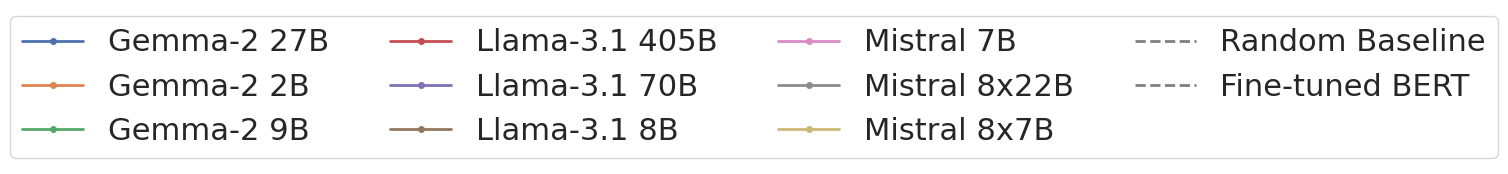
\includegraphics[width=0.95\textwidth]{figures/legend}
        \vspace{-3mm}
    \end{subfigure}\\
    \begin{subfigure}[b]{0.217\textwidth}
    \centering
    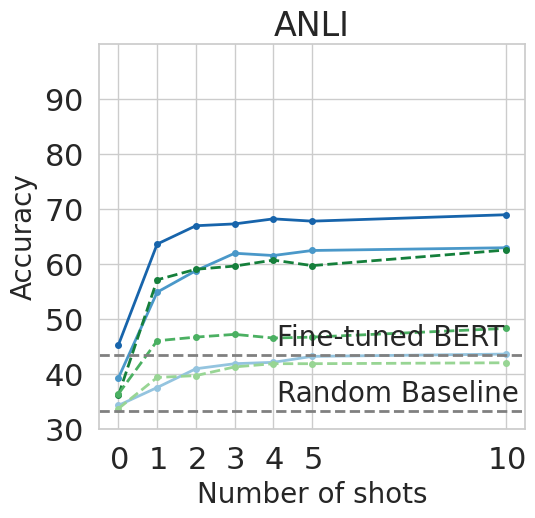
\includegraphics[height=3.45cm]{figures/anli}
    \caption{ANLI}
    \end{subfigure}
    \label{fig:anli}
    \begin{subfigure}[b]{0.19\textwidth}
    \centering
    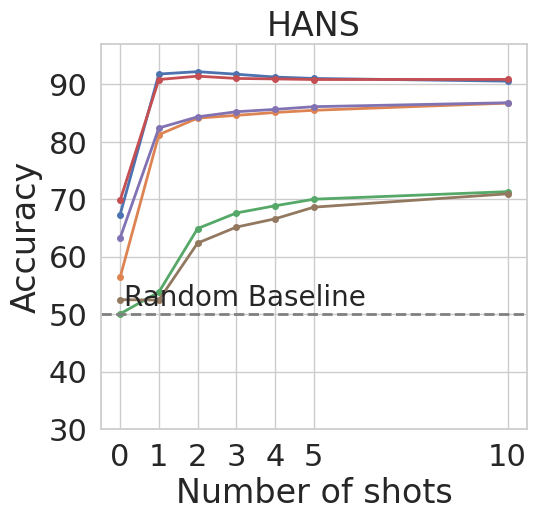
\includegraphics[height=3.45cm, trim=25mm 0 0 0, clip]{figures/hansnli}
    \caption{HANS}
    \label{fig:hans}
    \end{subfigure}
    \begin{subfigure}[b]{0.19\textwidth}
    \centering
    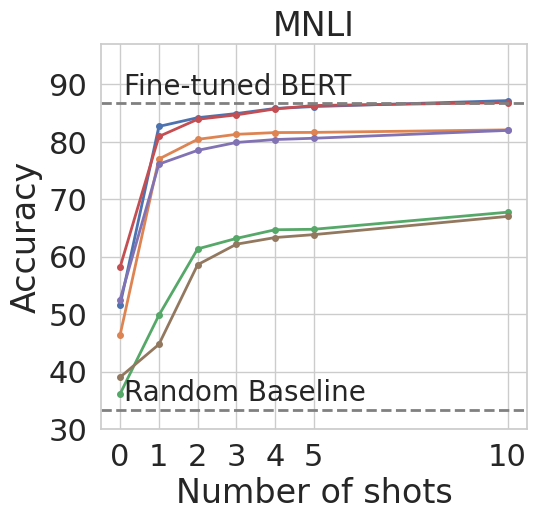
\includegraphics[height=3.45cm, trim=25mm 0 0 0, clip]{figures/mnli_matched}
    \caption{MNLI}
    \label{fig:mnli}
    \end{subfigure}
    \begin{subfigure}[b]{0.19\textwidth}
    \centering
    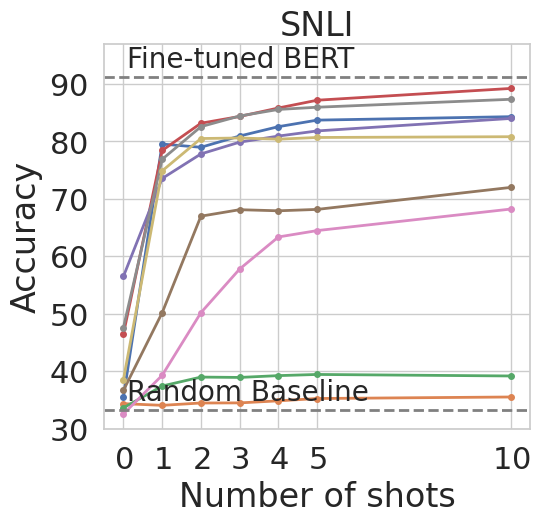
\includegraphics[height=3.45cm, trim=25mm 0 0 0, clip]{figures/snli}
    \caption{SNLI}
    \label{fig:snli}
    \end{subfigure}
    \begin{subfigure}[b]{0.19\textwidth}
    \centering
    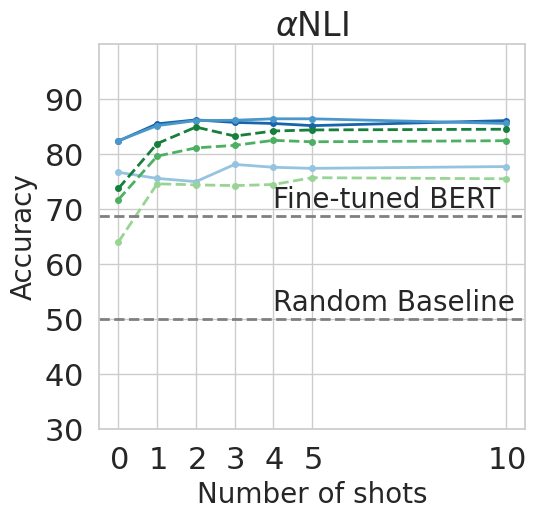
\includegraphics[height=3.45cm, trim=25mm 0 0 0, clip]{figures/abductivenli}
    \caption{$\alpha$NLI}
    \label{fig:alphanli}
    \end{subfigure}
    \caption{\textbf{Performance across shots.} We show performance across shots for nine trained-out models, for ANLI, HANS, MNLI, SNLI and $\alpha$NLI. Dashed lines indicate Random, and Finetuned-BERT baselines.}\label{fig:shot_performance}
\end{figure*}

% \paragraph{Q1: Does NLI provide signal for LLMs?}
% We show \begin{enumerate}
%     \item curves + scores on trained-out models.  Conclusion: ? Should say something about whether it is separating models in early stages of training, and whether it is monotonic, how much variance etc.
%     \item Trained out model scores. Tentative conclusion (pending numbers): with the exception of abductive NLI, these datasets allow to distiguish models of different sizes. Doesn't work at all with zero-shot (which can explain some previous results?), but with one or two shots we get decent scores. ANLI seems to be the most challenging with around 70\% accuracy on the 405B model.
%     \item Ablations: conclusion??
% \end{enumerate}

With the goal to get an overall estimate of the difficulty of the task and the extent to which it can discriminate models, we first consider the performance of fully pre-trained models from the respective model series.

\paragraph{Accuracy across shots}
For each of the models, we compute results with variable number of shots.
We report the results in \cref{fig:shot_performance}, along with a chance baseline and the results of a fine-tuned BERT model.
For all models, we observe rather poor zero-shot performance for all tasks, except $\alpha$NLI, confirming previously reported results by \citet{ohmer2024form} and \citet{weber-etal-2023-mind}, among others.
When more shots are added, performance starkly improves.
Even with just one shot, the performance is significantly better than the zero shot accuracy.
Adding more than three or four examples in the few shots does not improve performance much and saturates around 10 shots. 
Among the five benchmarks, the most challenging benchmark is ANLI.
Although the larger models in the Llama and Mistral series far outperform the finetuned BERT baseline, they do not exceed 70\% accuracy -- to some extent confirming the difficulty of the benchmark reported by \citet{brown2020language}.

\paragraph{Model discriminability}
In terms of discriminability, virtually all benchmarks provide a clear gap between the smaller and larger models for both families of models we consider.
For example, for the Llama series, 405B performs the best followed by 70B and then the 8B.
Though these three models are trained on the same amount of text tokens, performance clearly improves with scale.
The exception to this pattern is $\alpha$NLI, which appears to be near-saturated already at 70B scale, at an accuracy of around 85\%.
We conclude, from these results, that the benchmarks under consideration provide a useful signal to compare trained-out models, though it is unclear to what extent their performance has saturated, a question that we discuss in more detail later in this paper (\cref{subsec:saturation}).
% Gemma-2 9B model has chance accuracy and has similar performance to the 2B model and does not show this scaling behaviour, but it's visible with the 27B model scale. This is not the case in its counterparts in the Mistral and Llama series, where the smaller models perform significantly better and the larger models in the respective model families are even better.

% \subsection{Performance development over training}
\subsection{Informativeness during training}\label{subsec:during_training}

Next, we investigate whether NLI datasets may provide a good signal during training.
To this end, we pre-train Llama-3 architecture-based 8B and 70B models from scratch for 2T tokens. For the pre-training datamix, we use a mix of data available from publicly available sources including web data, code, and reasoning datasets.

\paragraph{Training curves} In \cref{fig:performance_training}, we show how (four-shot) performance develops during training.
We see that for most benchmarks, the 8B and 70B model quickly start to diverge.
The 70B model starts improving after around 250B tokens, for ANLI and $\alpha$NLI, it crosses fine-tuned BERT performance after around 500B tokens.
On the other hand, the development of performance for the 8B model is slow, at this scale not exceeding chance accuracy for HANS, MNLI, and SNLI.
From the final model performance of 8B depicted in \cref{fig:shot_performance}, we can conclude that the 8B model improves fairly late during the training stage.
We did not have the budget to do the full pre-training run, but longer training definitely seems to help on NLI tasks, further confirming the claim that NLI models can still provide a helpful signal.

\begin{figure*}[t]
    % \begin{subfigure}[b]{\textwidth}
    %     %\centering
    %     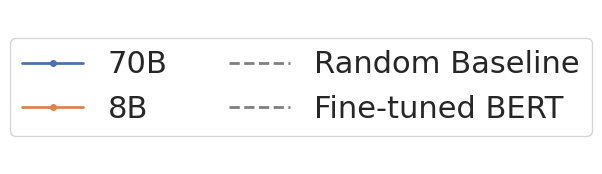
\includegraphics[width=0.3\textwidth]{figures/training_legend}
    %     \vspace{-2mm}
    % \end{subfigure}\\
    \begin{subfigure}[b]{0.20\textwidth}
    \centering
    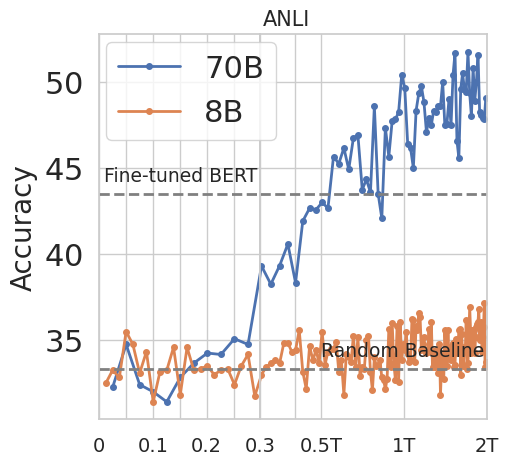
\includegraphics[height=3.2cm]{figures/anli_intermediate}
    \caption{ANLI}
    \end{subfigure}
    \label{fig:anli_int}
    \begin{subfigure}[b]{0.19\textwidth}
    \centering
    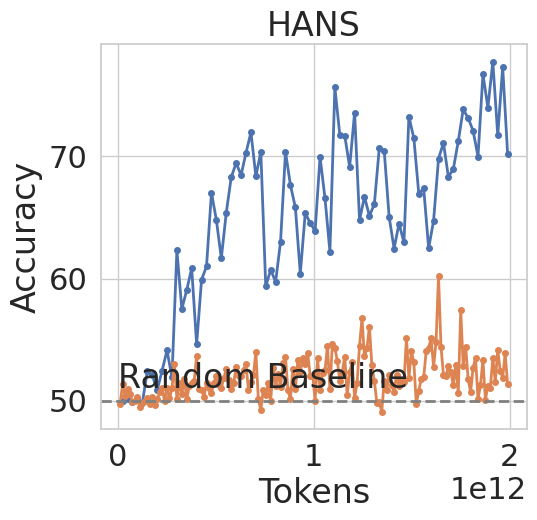
\includegraphics[height=3.2cm, trim=11mm 0 0 0, clip]{figures/hansnli_intermediate}
    \caption{HANS}
    \label{fig:hans_int}
    \end{subfigure}
    \begin{subfigure}[b]{0.19\textwidth}
    \centering
    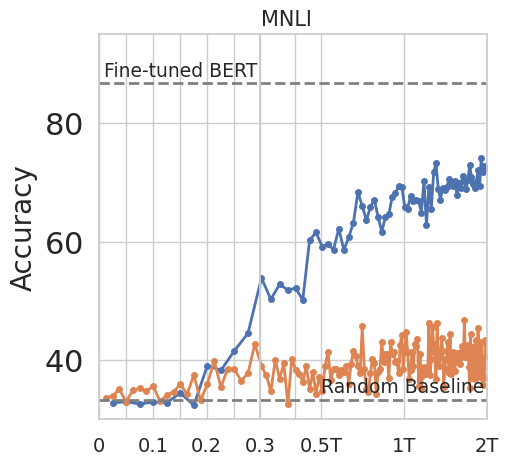
\includegraphics[height=3.2cm, trim=11mm 0 0 0, clip]{figures/mnli_matched_intermediate}
    \caption{MNLI}
    \label{fig:mnli_int}
    \end{subfigure}
    \begin{subfigure}[b]{0.19\textwidth}
    \centering
    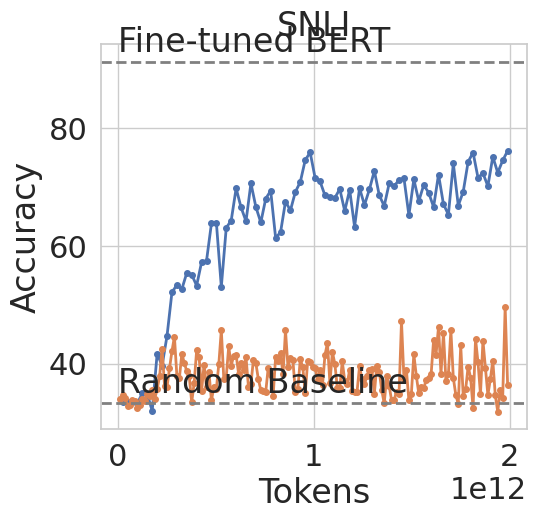
\includegraphics[height=3.2cm, trim=11mm 0 0 0, clip]{figures/snli_intermediate}
    \caption{SNLI}
    \label{fig:snli_int}
    \end{subfigure}
    \begin{subfigure}[b]{0.19\textwidth}
    \centering
    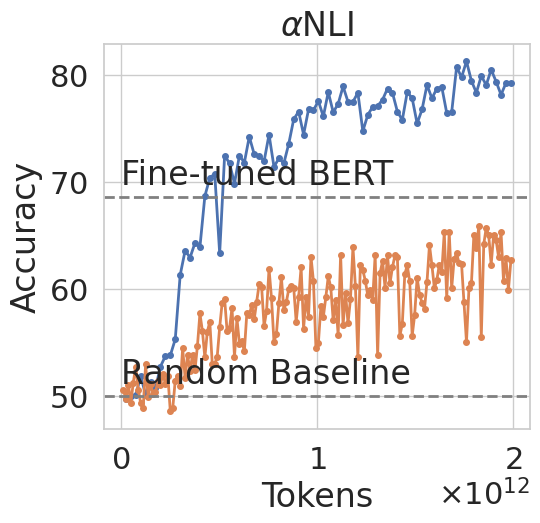
\includegraphics[height=3.2cm, trim=11mm 0 0 0, clip]{figures/abductivenli_intermediate}
    \caption{$\alpha$NLI}
    \label{fig:alphanli_int}
    \end{subfigure}
    \caption{\textbf{Performance during training.} We show how performance for the five benchmarks develops during training, for two Llama-3 style models.}\label{fig:performance_training}
\end{figure*}

\paragraph{Utility for ablations}
A requirement for a benchmark to provide a useful signal during training is that it develops relatively monotonically during training.
The plots in \cref{fig:performance_training} suggest that this is not the case for most of the benchmarks for the 8B model.
Following \citet{variancepaper}, we quantify the benchmarks' monotonicity on both a discrete (accuracy) and continuous metric (NLL).%
\footnote{Tracking continuous metrics like negative log likelihood (NLL) over the course of the training generally provides more monotonic results than discrete metrics such as accuracy.}
In \cref{tab:monotonicity}, we can see that, despite the benchmarks' moderate sizes, monotonicity is low for accuracy as well as NLL, suggesting that the benchmark may not be suitable for monitoring performance on small number of closely-spaced checkpoints at this scale. %for smaller models. 
% Monotonicity for the 70B is substantially higher for some benchmarks, but the compute involved for doing ablations increases 10x for stable signals.

\begin{table}
\centering
\resizebox{0.45\textwidth}{!}{
\begin{tabular}{lcccc}
    %\toprule
    %Model $\rightarrow$ 
    & \multicolumn{2}{c}{8B} & \multicolumn{2}{c}{70B} \\
    % \toprule
    %Benchmark $\downarrow$
    & $mon_{ACC}$  & $mon_{NLL}$ & $mon_{ACC}$ & $mon_{NLL}$ \\
    \toprule
    $\alpha$NLI & 0.62 & 0.62 & 0.79 & 0.79 \\
    \midrule
    ANLI & - & - & 0.67 & 0.47 \\
    \midrule
    HANS & 0.32 & 0.46 & 0.57 & 0.63 \\
    \midrule
    MNLI & 0.34 & 0.51 & 0.77 & 0.80 \\
    \midrule
    SNLI & 0.05 & 0.38 & 0.64 & 0.65 \\
    \bottomrule
    \end{tabular}
}
\caption{\textbf{Monotonicity values.} Monotonicity values for the 8B and 70B models during the course of the training. We report both the discrete ($mon_{ACC}$) and continuous ($mon_{NLL}$) monotonicity values. ACC and NLL represent Accuracy and Negative Log Likelihood respectively.}
\label{tab:monotonicity}
\end{table}

\subsection{Dataset saturation}\label{subsec:saturation}
Having confirmed that the NLI benchmarks under scrutiny provide discrimination between LLMs of different sizes, we now turn to the question of saturation: the results show that the benchmarks would have been useful so far, but how about the future?
As already pointed out before, the benchmark that still has the clearest room for improvement is adversarial benchmark ANLI, with performances not exceeding 70\% even for the largest models.
For the other benchmarks, performances are substantially higher, and it is unclear to what extent the benchmarks may suffer saturation.

\begin{table*}[h!]
\centering
\small
\resizebox{\textwidth}{!}{
\begin{tabular}{p{10.1cm}|c|c|c}
\toprule
\textbf{Example} & \textbf{Label distribution} & \textbf{Gold} & \textbf{Prediction} \\
\midrule
%\textbf{Premise}: Savonarola burned in Florence\\
%\textbf{Hypothesis}: Florence became Savonarola's new home. & e: 3, n: 40, \textbf{c: 57} & c & n \\
%\midrule
    \makecell[l]{
    \textbf{Premise}: of course you could annex Cuba but they wouldn't like that a bit\\
    \textbf{Hypothesis}: Annexing Cuba is a great idea.
    } & e: 0, n: 31, \textbf{c: 69} & c & n \\
\midrule
\makecell[l]{
    \textbf{Premise}: I thought working on Liddy's campaign would be better than working\\ on Bob's. \\
    \textbf{Hypothesis}: I thought I would like working on Liddy's campaign the best.
    } & \textbf{e: 66}, n: 32, c: 2 & n & e \\
% \textbf{Premise}: you want to punch the button and go\\
% \textbf{Hypothesis}: You don't want to push the button lightly, but rather punch it hard. & \textbf{e: 48}, n: 45, c: 7 & n & n \\
% \midrule
\midrule
\makecell[l]{
\textbf{Premise}: Sorry but that's how it is.\\
\textbf{Hypothesis}: This is how things are and there are no apologies about it.
    }& \textbf{e: 48}, c: 40, n: 12 & c & c \\
\bottomrule
\end{tabular}
    }
    \caption{\textbf{Examples from ChaosNLI with different label distributions.} We show different samples from ChaosNLI with different annotator distributions. The first column shows the example; the second the distribution of human labels across the 100 collected annotations (the majority label is marked bold), the third column indicates the label that the example had in the original dataset and the fourth column the Llama 3.1 405B prediction.}
\label{tab:sample_analysis}
\end{table*}

\paragraph{Error types} To address this question, we first conduct a manual error analysis on the examples that the largest models assign an incorrect label.
Specifically, we focus on one MNLI, one of the datasets with the highest scores, and analyse the predictions of Llama 3.1 405B model.
In \cref{tab:sample_analysis}, we show a few examples, along with 100 human annotations for that sample from the previously mentioned dataset ChaosNLI.
For all the examples we looked at, we found that there was at least some degree of interpretation or ambiguity in assigning a label to the premise-hypothesis pair.
For example, in the first row of \cref{tab:sample_analysis}, whether the correct label is contradiction or negation would depend on a not-specified sentiment towards Cuba.
In fact, 31 out of 100 human annotators would agree with the model's judgement.
Also in the second row of \cref{tab:sample_analysis}, we see an example where human opinions diverge on what the correct label is.
In this case, the model's prediction matches the majority label found by \citet{nie-etal-2020-learn}, but the sample is marked incorrect because the MNLI label is a different one.
It is worth pointing out, that the same is sometimes true for examples that are marked \emph{correct}.
Consider, for instance, the last row in \cref{tab:sample_analysis}, where the model prediction matches the gold label in the MNLI dataset, but not the majority label collected by ChaosNLI.
In sum, it appears that for the best model, most of the `mistakes' in MNLI are cases in which humans may not agree on the correct label.

\paragraph{Majority accuracy} 
Next, we study this phenomenon more quantitatively, again utilising the ChaosNLI dataset, which contains 100 human annotations for over 1500 samples of the datasets MNLI, SNLI and $\alpha$NLI, each.
First, we consider how models' accuracies changes when we replace the original labels with the majority label of the ChaosNLI dataset.
This changes 32\%, 25\% and 11\% of the labels of MNLI, SNLI and $\alpha$NLI, respectively.
In Table \ref{tab:chaos_acc}, we can see that the results differ per model and benchmark.
The largest effects are observed for MNLI, where for some models an increase of more than 10\% point is observed and the average accuracy across models is more than five points higher on the `corrected' datasets.
For the other two benchmarks, the results are more mixed, with little to no difference on average.
Only for the largest Llama-3.1 model (405B), the majority accuracy is systematically higher than the original accuracy, suggesting it may have honed in more on the majority label.
Interestingly, the MNLI and SNLI subsets of ChaosNLI appear substantially more difficult than the average dataset;
Even the Llama3.1 405B model stays below 70\% on both these subsets, suggesting that there is room for improvement on both these datasets.

\begin{table*}
    \centering
    \begin{tabular}{llcccccc}
        & & \multicolumn{2}{c}{\textbf{$\alpha$NLI}} & \multicolumn{2}{c}{\textbf{MNLI}} & \multicolumn{2}{c}{\textbf{SNLI}} \\
        \multicolumn{2}{c}{\textbf{Model}} & \textit{Og.} & \textit{Maj.} & \textit{Og.} & \textit{Maj.} & \textit{Og.} & \textit{Maj.}\\
        \toprule
        Llama-3.1 & 8B & 77.55 & \textbf{78.00} & 49.47 & \textbf{50.97} & \textbf{55.28} & 55.48 \\
        Llama-3.1 & 70B & 86.36 & \textbf{87.21} & 57.66 & \textbf{67.54} & \textbf{60.44} & 58.52 \\
        Llama-3.1 & 405B & 85.51 & \textbf{86.10} & 64.04 & \textbf{69.67} & 64.60 & \textbf{67.31} \\
        \midrule
        Mistral & 7B & 74.41 & \textbf{75.78} & 49.97 & \textbf{53.22} & \textbf{49.47} & 48.15 \\
        Mixtral & 8x7B & \textbf{82.44} & 81.59 & \textbf{54.03} & 51.53 & 63.14 & \textbf{64.27} \\
        Mixtral & 8x22B & \textbf{84.14} & 83.68 & 60.23 & \textbf{67.04} & 64.86 & \textbf{67.83} \\
        \midrule
        \multicolumn{2}{c}{\emph{Average}} & 76.01 & 76.21 & 50.86 & 55.93 & 54.90 & 54.35 \\
    \bottomrule
    \end{tabular}
    \caption{\textbf{Majority accuracy.} For each model and dataset, we show the accuracy on the ChaosNLI subsets of $\alpha$NLI, MNLI and SNLI. The original accuracy (Og.) represents the accuracy as computed according to the original labels of the respective datasets; the majority accuracy (Maj.) expresses accuracy according to the majority label.}
\label{tab:chaos_acc}
\end{table*}

\paragraph{Accuracy versus entropy}
Next, we consider the distribution of accuracy with entropy for the three benchmarks in Figure \ref{fig:entropy_accuracy}. We only show the smallest (8B) and the largest (405B) model in the Llama series across the three benchmarks. We observe that for the largest model, there's a clear decreasing trend of accuracy with increasing entropy for all three benchmarks, whereas for the 8B model, the trend is not that prominent and some entropy bins have similar accuracies. For the entropy vs accuracy distributions on other models, we refer the reader to Appendix \ref{sec:appendix}.

\begin{figure*}[t]
    \centering
    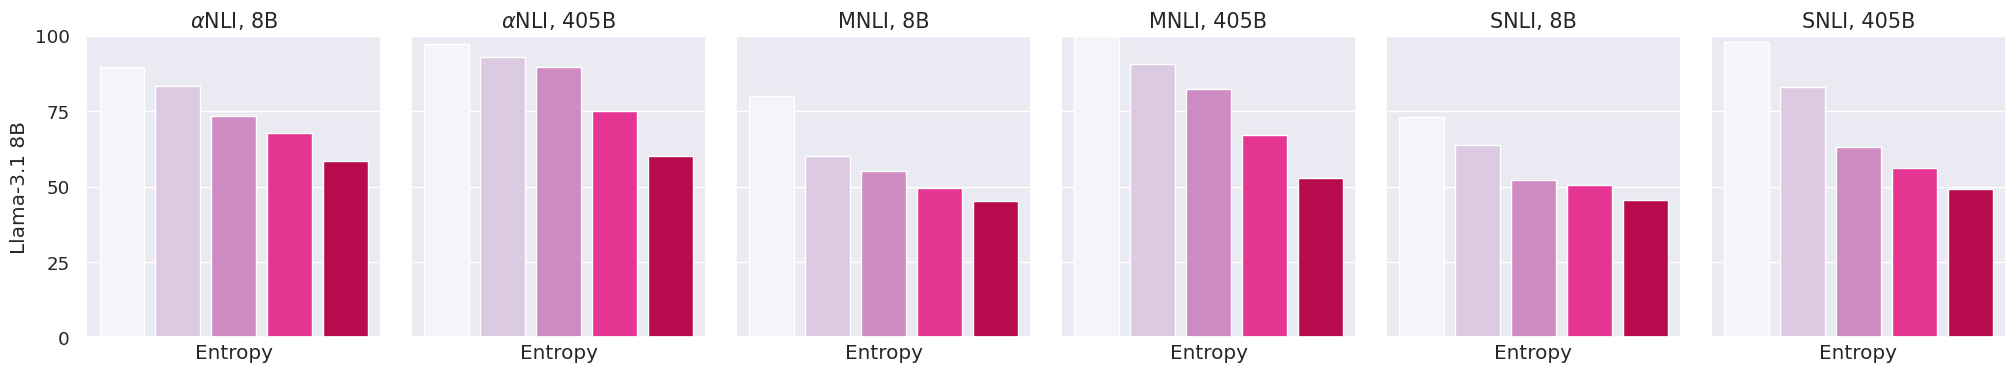
\includegraphics[width=0.95\linewidth]{figures/entropy_acc_8_405}
    \caption{\textbf{Accuracy versus entropy.} We show how the accuracy of Llama 8B and Llama 405B changes as the entropy of the human label distributions increases. Accuracy-vs-entropy plots for all other models can be found in \cref{fig:acc_vs_entropy_all}.}
    \label{fig:entropy_accuracy}
\end{figure*}

In \cref{fig:entropy_accuracy}, we can furthermore see that all models perform `better' on samples where the entropy of the labels is low.
For the larger models, this effect is larger: on samples where humans have high disagreement (and the majority label is thus in a way more representative of the average human judgements), their accuracies are often near maximal, and they drop down as human judgements become more dispersed.

\paragraph{Implications for saturation}
What the implication of these results is for the question of saturation of these benchmarks is, like the samples of the benchmark themselves, open to interpretation.
On the one hand, it appears that in several cases, the model's predictions do not align with the human majority label, suggesting that the performance may still improve as models continue training.
On the other, the results put into question whether strong alignment with the majority label is in fact what we should strive for: if humans have low agreement on their judgements, should the desired behaviour of a model really be to only align with the majority?
In the next section, we approach this question by considering the distribution of model outputs, rather than only the highest probability label.

% Benchmark: mnli_matched
% Number of examples: 1599
% Number of flipped labels: 508
% Number of same labels: 1091
% Percentage of flipped labels: 31.77
% 
% Benchmark: snli
% Number of examples: 1514
% Number of flipped labels: 378
% Number of same labels: 1136
% Percentage of flipped labels: 24.97
% 
% Benchmark: abductivenli
% Number of examples: 1532
% Number of flipped labels: 163
% Number of same labels: 1369
% Percentage of flipped labels: 10.64

% To further investigate the phenomenon observed in the previous subsection, we more intensively utilise the dataset ChaosNLI \citep{nie-etal-2020-learn}, which contains 100 human annotations for over 1500 samples of the datasets MNLI, SNLI and $\alpha$NLI, each.
% Using this data, we can i) estimate the extent to which suboptimal performances are due to cases where the dataset label does not match the majority label, and ii) investigate how model judgements change as human uncertainty on the task increases.

\subsection{Model versus human distributions}\label{subsec:chaosnli_dist}
The ChaosNLI dataset does not only help us estimate the adequacy of the original label sets of the respective datasets, it also allows us to study how models behave in scenarios where there is not a single, correct, ground-truth answer.
In a time where LLMs are employed simultaneously to many users with potentially different preferences, this question has become very practically relevant.
To do so, we consider how the probability distribution of the models over the three possible labels \textit{Entailment}, \textit{Neutral}, and \textit{Contradiction}) compares with the label distributions observed in the human annotations.
Following \citet{nie-etal-2020-learn}, we consider Jensen-Shannon Divergence \citep[JSD][]{menendez1997jensen} to measure the distance between the two distributions. 
%Mathematically,
%
%\[
%    JSD(p || q) = \sqrt{\frac{1}{2}KL(p || m) + \frac{1}{2}KL(q || m)},
%\]
%
%where $p$ is the human annotator distribution, $q$ is the softmax probability distribution, and $m = \frac{1}{2}(p + q)$. 
Contrary to Kullback Leibner (KL) divergence, JSD is symmetric and bound between 0 and 1, making it more interpretable for our specific case.

\begin{figure*}[t]
    % \begin{subfigure}[b]{\textwidth}
    %     %\centering
    %     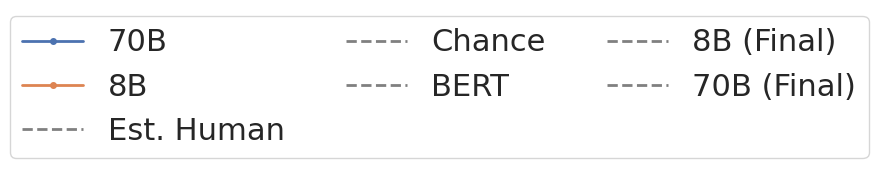
\includegraphics[width=0.2\textwidth]{figures/chaos_jsd_training_legend}
    %     % \vspace{-2mm}
    % \end{subfigure}\\
    \begin{subfigure}[b]{0.32\textwidth}
        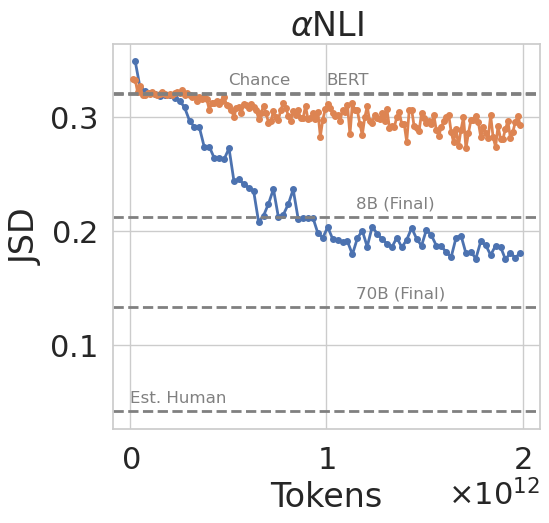
\includegraphics[height=4.5cm]{figures/abductivenli_intermediate_jsd}
        \caption{}
    \end{subfigure}
    \begin{subfigure}[b]{0.32\textwidth}
        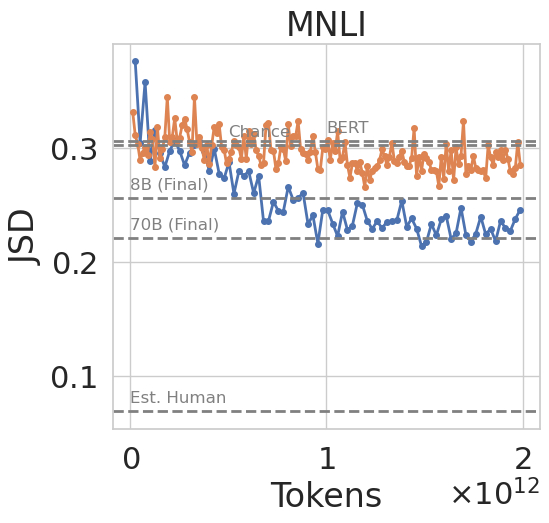
\includegraphics[height=4.5cm, trim=11mm 0 0 0, clip]{figures/mnli_matched_intermediate_jsd}
        \caption{}
    \end{subfigure}
    \begin{subfigure}[b]{0.32\textwidth}
        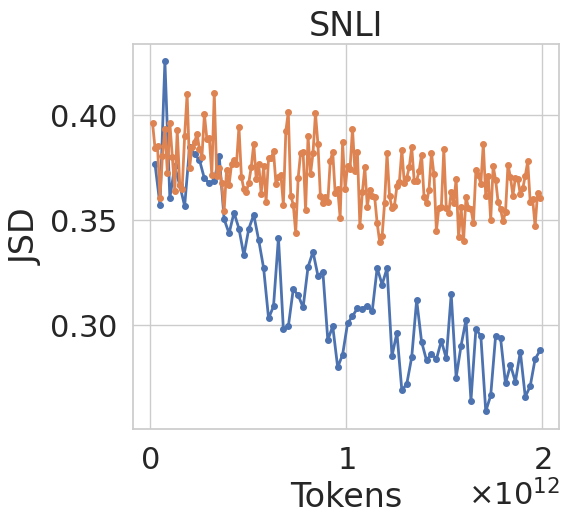
\includegraphics[height=4.5cm, trim=11mm 0 0 0, clip]{figures/snli_intermediate_jsd}
        \caption{}
    \end{subfigure}
    \caption{\textbf{Development of JSD during training.} We show how the JSD of our trained-from-scratch 8B and 70B model develops during training.}\label{fig:jsd_training}
\end{figure*}

In \cref{fig:jsd_all_benchmarks}, we can see that, for MNLI, all considered models have probability distributions more similar to the human distributions than chance, but substantially more different than humans have among each other.\footnote{The human estimate was computed by \citet{nie-etal-2020-learn}, on an independent sample of human annotations on the same data.}
This pattern is constant across datasets.
Interestingly, larger models appear to have lower divergence, contradicting the finding of \citet{nie-etal-2020-learn} that better or larger models do not have more similar distributions.
Yet, the effect of scale is further confirmed in \cref{fig:jsd_training}: though even trained-out models are far away from a low JSD, the JSD of the model softmax distributions and the human label distributions goes down steadily during training.
This is an exciting finding, because it suggests that measuring similarity with human distributions could be an interesting venue to explore during training.

\begin{figure*}
    \centering
    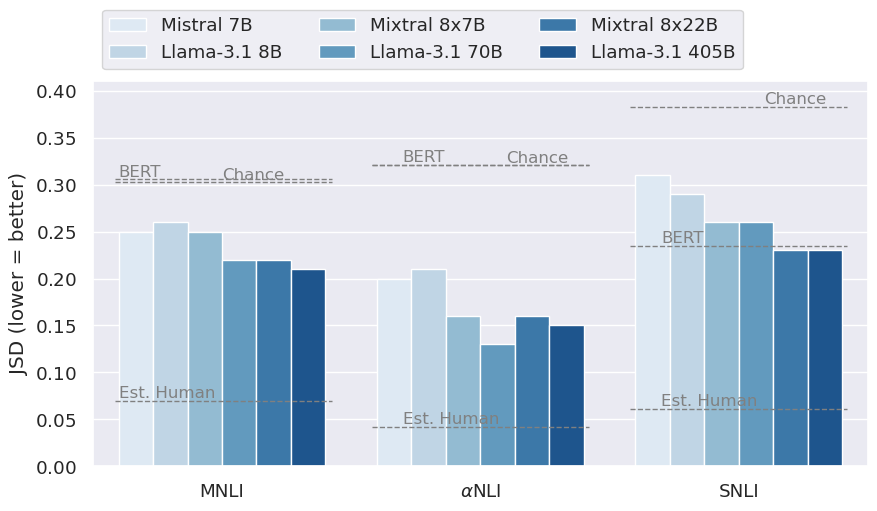
\includegraphics[width=0.6\linewidth]{figures/jsd_all_benchmarks}
    \caption{Final model JSDs for each of the benchmarks in ChaosNLI.}
    \label{fig:jsd_all_benchmarks}
\end{figure*}
% 
% \begin{figure*}
%     \centering
%     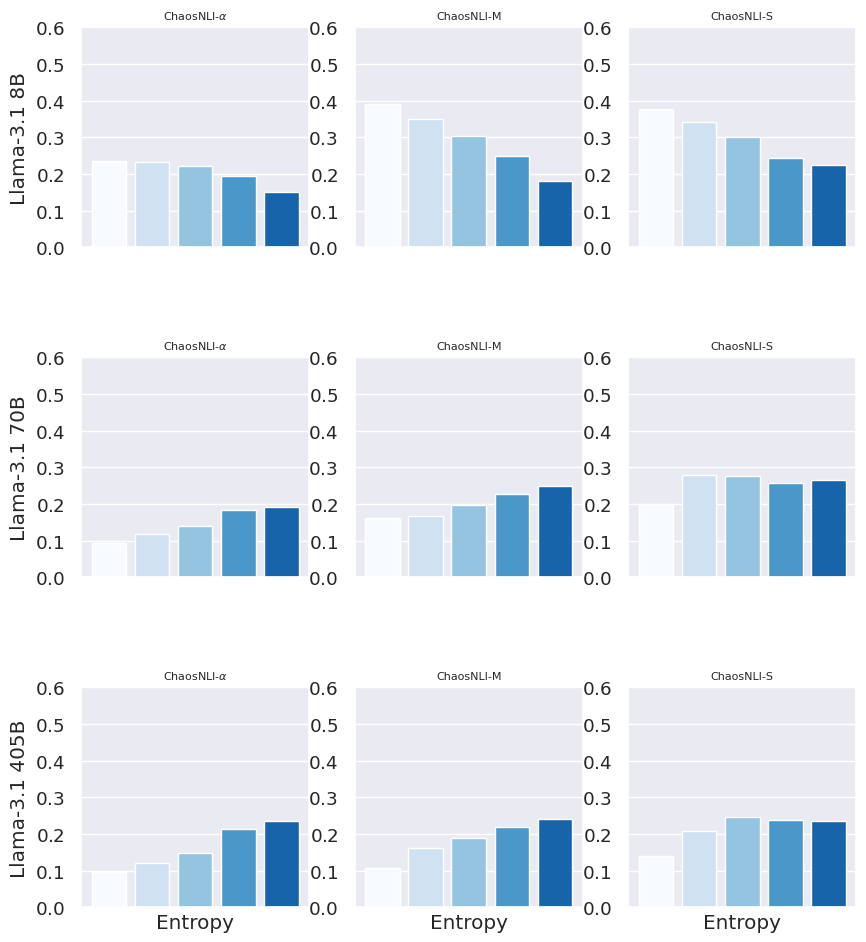
\includegraphics[width=0.7\linewidth]{figures/entropy_jsd.png}
%     \caption{JSD vs entropy plots for the Llama series of models for the three subsets in ChaosNLI.}
%     \label{fig:entropy_jsd}
% \end{figure*}

\subsection{Contamination Analysis}\label{subsec:contamination}

Now that we've concluded that NLI benchmarks provide a signal both for final models and during pre-training, we perform a contamination analysis for all the benchmarks considered.
 % , to ensure that the performance we observe is solely due to better training paradigm, data, and model architectures, and not just because of contamination in the pre-training data mixture.
Using the methodology used by \citep{dubey2024llama}, we analyse contamination assigning a score to each evaluation sample which represents the percentage of tokens in the sample that is part of an 8-gram occurring in the pretraining dataset.
We select contamination thresholds considering the estimated performance gain (EPG) for each threshold.
A threshold of 0 leads to all examples having non-zero contamination scores to be marked as contaminated and as we increase the threshold, examples are moved to the `uncontaminated' subset.
In \cref{fig:contamination}, we plot the EPG as a function of the percentage of the data that is marked contaminated according to a given contamination threshold.

\begin{figure*}[t]
    \begin{subfigure}[b]{0.20\textwidth}
    \centering
    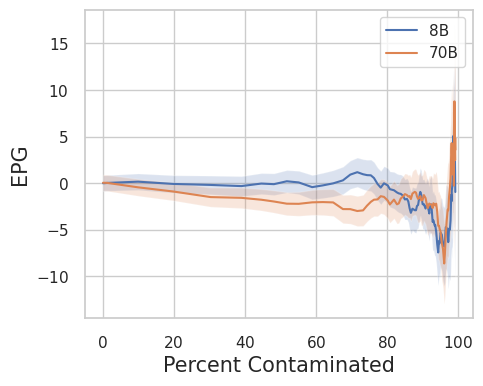
\includegraphics[height=2.7cm]{figures/contamination_anli}
    \caption{ANLI}
    \end{subfigure}
    \label{fig:cont_anli}
    \begin{subfigure}[b]{0.19\textwidth}
    \centering
    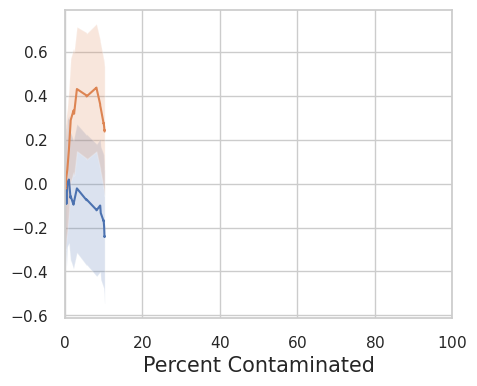
\includegraphics[height=2.7cm]{figures/contamination_hansnli}
    \caption{HANS}
    \label{fig:cont_hans}
    \end{subfigure}
    \begin{subfigure}[b]{0.19\textwidth}
    \centering
    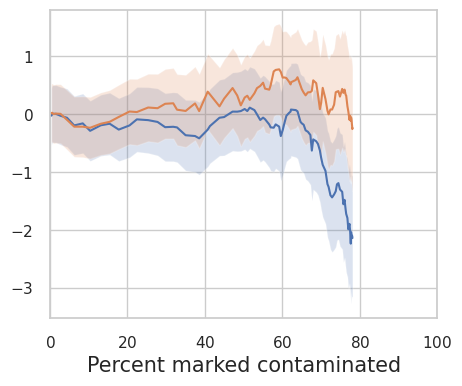
\includegraphics[height=2.7cm]{figures/contamination_mnli_matched}
    \caption{MNLI}
    \label{fig:cont_mnli}
    \end{subfigure}
    \begin{subfigure}[b]{0.19\textwidth}
    \centering
    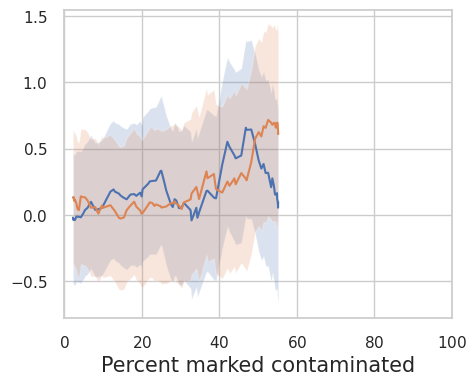
\includegraphics[height=2.7cm]{figures/contamination_snli}
    \caption{SNLI}
    \label{fig:cont_snli}
    \end{subfigure}
    \begin{subfigure}[b]{0.19\textwidth}
    \centering
    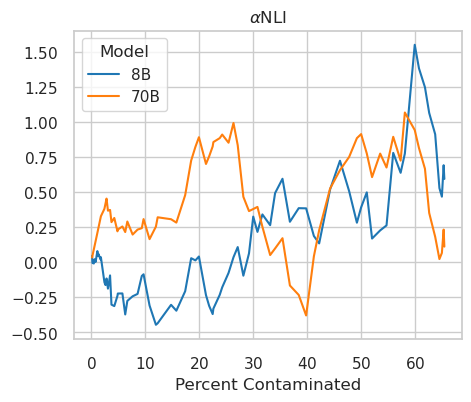
\includegraphics[height=2.7cm]{figures/contamination_abductivenli}
    \caption{$\alpha$NLI}
    \label{fig:cont_alphanli}
    \end{subfigure}
    \caption{\textbf{Contamination Scores.} TODO}\label{fig:contamination}
\end{figure*}

% We plot the ``Estimated Performance Gain'' (EPG) for the two models we trained from scratch. EPG is defined as the difference in performance on the entire subset and the `uncontaminated' subset. 
% We plot it versus the percent contamination determined according to a given contamination threshold. 

In \cref{fig:contamination}, we can see that there is virtually no score inflation as a consequence of contamination for the 8 and 780B model that we considered.
For HANS, this is because virtually no contamination is detected by 8-gram overlap.
For MNLI, SNLI and $\alpha$NLI, instead, large parts of the dataset are marked contaminated at low thresholds, but there is no performance impact.
We suspect that this is because the premises of the samples are sourced from publicly available datasets, and their presence per se is thus not indicitive of contamination.
Likely for similar reasons, almost all of the ANLI samples contain at least one overlapping 8-gram, resulting in very high percentages of detected contamination at low thresholds.
As the `clean' partition of the dataset at these thresholds is low, it is not possible to determine whether these samples may constitute only false positives, as illustrated also by the erratic behaviour of the EPG in \cref{fig:contamination}. 
% observe that HANS has negligible contamination as the maximum percentage contamination is around 10\%, whereas the other benchmarks have a significant amount of contamination. 
% But, the contamination does not help in the case of MNLI, SNLI, and $\alpha$NLI benchmarks, as EPG hovers around 0. 
% For ANLI, even though there's a lot of contamination (probably since ANLI is derived from news articles and pre-training mix has a lot of news articles), both the 8B and 70B are not able to exploit the contamination because EPG increases only when we keep the threshold for contamination close to 0.
% 
Thus, we believe that contamination does not play a participatory role in models being good at NLI benchmarks, and ANLI is the most challenging out of the five benchmarks we consider.


\section{Conclusion}

In this work, we revisit natural language inference (NLI) benchmarks and investigate if they may still play a role in LLM evaluation, both during and after pre-training.
We consider five different NLI benchmarks -- $\alpha$NLI, ANLI, HANS, and MNLI -- and evaluate them across six different models of two model families: Llama 3.1 8B, 70B, and 405B, and Mistral 7B, 8x7B, and 8x22B.
Furthermore, we consider how the benchmark behave during the training of two Llama-style 8B and 70B models.
We find that, with the exception of $\alpha$NLI, all benchmarks are able to discriminate between models of different qualities, and in particular ANLI is challenging even for the largest models.
Furthermore, we find next to no effect of contamination for the benchmarks.
Considering the benchmark ChaosNLI \citep{nie-etal-2020-learn}, containing 100 human annotations for over 4500 samples of three of the benchmarks we consider, we also find that the differences between human label distributions and model label distributions -- as measured with Jensen Shannon Divergence (JSD) -- has decreased for the new generation of models.
However, they are still substantially higher than the distributional difference between two populations of humans. 
Interestingly, contrary to the findings of \citet{nie-etal-2020-learn}, we observe a clear effect of scale.
JSD shows a steady decrease during training, and larger models have lower JSD than smaller models, making it a potentially interesting quality to consider for model development.


\section{Limitations}

One of the limitation of our work is that all our analysis is limited to pre-trained models. Post-training with supervised fine-tuning and RLHF might change the behaviour of models on NLI benchmarks. But, we do not believe this to be a major limitation as \citet{dubey2024llama} show that it's possible to improve the performance of models during the post-training phase, rather than lose it because of instruction fine-tuning and safety.

% \clearpage

% Bibliography entries for the entire Anthology, followed by custom entries
\bibliography{anthology,custom}
% Custom bibliography entries only
% \bibliography{custom}

\appendix

\onecolumn
\section{Benchmarks}
\label{app:benchmarks}

Below, we provide a more elaborate description of (construction of) the benchmarks we consider in our work.
A summary of their statistics can be found in \cref{tab:dataset}.

\begin{table}
\centering
\begin{tabular}{c|c|c}
    Benchmark & \# Samples & \# labels \\
    \hline
    ANLI & 1200 & 3 \\
    HANS & 30000 & 2 \\
    MNLI & 9815 & 3 \\
    SNLI & 9842 & 3 \\
    $\alpha$NLI & 1532 & 2 \\
\end{tabular}
\caption{Dataset details}
\label{tab:dataset}
\end{table}

\subsection{SNLI}
Introduced by \citet{bowman-etal-2015-large}, the Stanford Natural Language Inference (SNLI) dataset was one of the first large-scale NLI dataset for NLP evaluation.
The dataset comprises of 570K human-authored English sentence pairs, sourced by asking Amazon Mechanical Turk workers to supply hypotheses for the three labels available in the dataset -- entailment, neutral and contradiction -- given a premise comprised by an image caption drawn from a pre-existing corpus.
For 57K of the resulting samples were then labeled by four additional annotators.
In this work, we consider the 10K development set of the corpus.
Like the original paper, we exclude samples for which no gold label exists because there was no label that three or more annotators agreed on.

\subsection{MNLI}
The Multi-Genre NLI (MNLI) corpus \citep{williams-etal-2018-broad} was introduced as an alternative to SNLI that captures more genres and more challenging examples, representing both written and spoken speech in a range of different styles, degrees, formalities, and topics.
The data collection procedure of the corpus is similar to the SNLI procedure both in terms of sourcing and validation.
Unlike SNLI, the MNLI premise sentences are derived from nine different sources, aiming to represent the full range of American English rather than a single image captioning corpus.
As for SNLI, we consider the validation corpus of the dataset and exclude samples that have no gold label.

\subsection{HANS}
Deviating from previous datasets, the adversarial dataset Heuristic Analysis for NLI Systems \citep[HANS,][]{mccoy-etal-2019-right} is not crowd-sourced, but synthetically generated using templates.
Specifically, the templates are designed to generate examples that can not be solved through heuristics such as lexical, subsequence, or constituent overlap.
At the time of proposal, none of the SOTA models were able to solve such examples.

\subsection{ANLI}
The second adversarial dataset we consider is Adversarial NLI \citep[or ANLI,][]{nie-etal-2020-adversarial}.
The dataset, created with the primary aim to make SOTA models fail, is sourced iteratively in a human-in-the-loop setup.
Given a premise and a target label, annotators are asked to propose hypotheses that may fool models.
The produced samples are then tested on a model, and the examples that do indeed receive an incorrect label are re-validated by one or more human validators.
The dataset consists of three sets of increasingly challenging examples, where in each round more powerful models are considered that are trained on examples from the previous round.
The third round furthermore contains a set of more diverse premises.
For our experiments, we are using the dev set of round 3, the most challenging set of the benchmark.

\subsection{$\alpha$NLI}
Differing in setup from the previously described benchmarks, $\alpha$NLI or abductive NLI \citep{bhagavatula2020abductive} focuses on \emph{abductive reasoning} -- which they describe as the inference of the most plausible explanation for an incomplete observation.
The samples in $\alpha$NLI consist of a pair of observations at two consecutive times, and a plausible hypothesis that explains tho two observations, and an implausible hypothesis that does not (or to a lesser extent).
The task is to select the most plausible hypothesis.
To construct the data \citet{bhagavatula2020abductive} first draw observation pairs from a stories dataset and then ask crowd-sources to generate plausible and implausible hypotheses. 
For each observation pair, multiple plausible and implausible hypotheses are crowd-sourced, and adversarial filtering is applied to retain one challenging pair of hypotheses.
We use the development set of the corpus for our experiments.



\section{Entropy vs accuracy plots}\label{app:entropy_vs_accuracy}

\begin{figure*}[t]
    \centering
    \begin{subfigure}[b]{0.23\textwidth}
        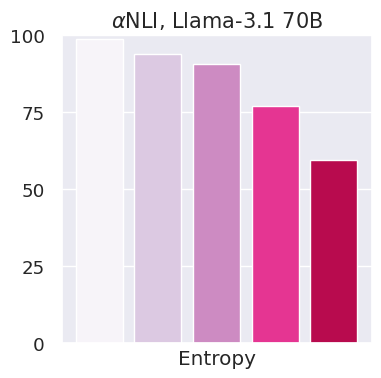
\includegraphics[height=3.6cm]{figures/appendix/entropy_acc_abductivenli_70B}
        % \caption{}
    \end{subfigure}
    \begin{subfigure}[b]{0.23\textwidth}
        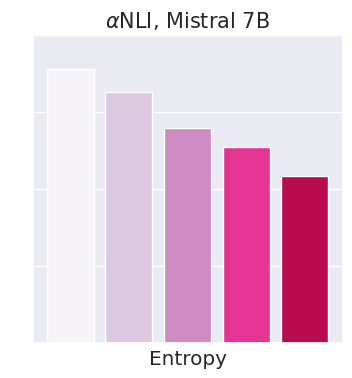
\includegraphics[height=3.6cm]{figures/appendix/entropy_acc_abductivenli_7B}
        % \caption{}
    \end{subfigure}
    \begin{subfigure}[b]{0.23\textwidth}
        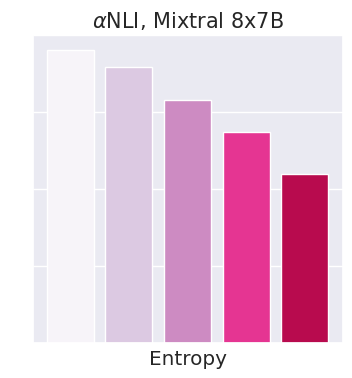
\includegraphics[height=3.6cm]{figures/appendix/entropy_acc_abductivenli_8x7B}
        % \caption{}
    \end{subfigure}
    \begin{subfigure}[b]{0.23\textwidth}
        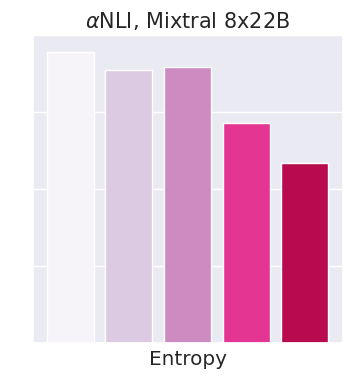
\includegraphics[height=3.6cm]{figures/appendix/entropy_acc_abductivenli_8x22B}
        % \caption{}
    \end{subfigure}\\
    \begin{subfigure}[b]{0.23\textwidth}
        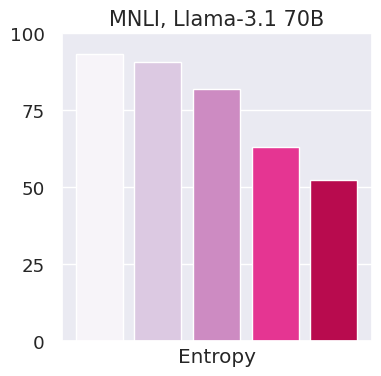
\includegraphics[height=3.6cm]{figures/appendix/entropy_acc_mnli_matched_70B}
        % \caption{}
    \end{subfigure}
    \begin{subfigure}[b]{0.23\textwidth}
        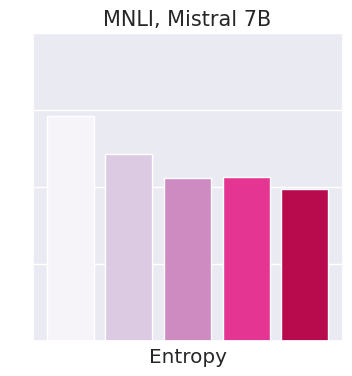
\includegraphics[height=3.6cm]{figures/appendix/entropy_acc_mnli_matched_7B}
        % \caption{}
    \end{subfigure}
    \begin{subfigure}[b]{0.23\textwidth}
        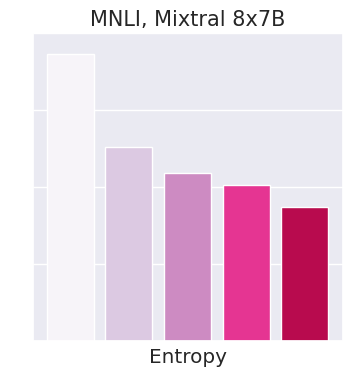
\includegraphics[height=3.6cm]{figures/appendix/entropy_acc_mnli_matched_8x7B}
        % \caption{}
    \end{subfigure}
    \begin{subfigure}[b]{0.23\textwidth}
        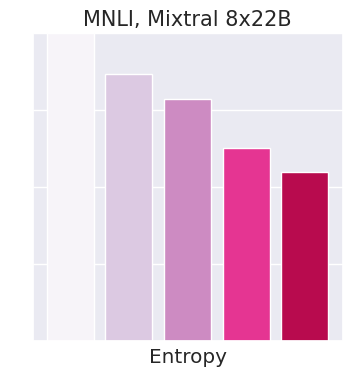
\includegraphics[height=3.6cm]{figures/appendix/entropy_acc_mnli_matched_8x22B}
        % \caption{}
    \end{subfigure}\\
    \begin{subfigure}[b]{0.23\textwidth}
        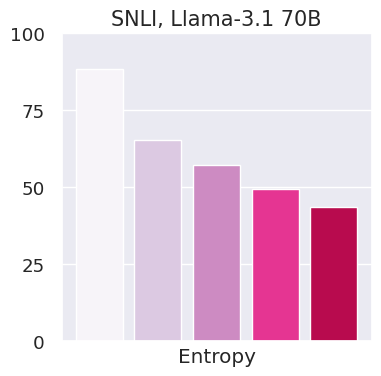
\includegraphics[height=3.6cm]{figures/appendix/entropy_acc_snli_70B}
        % \caption{}
    \end{subfigure}
    \begin{subfigure}[b]{0.23\textwidth}
        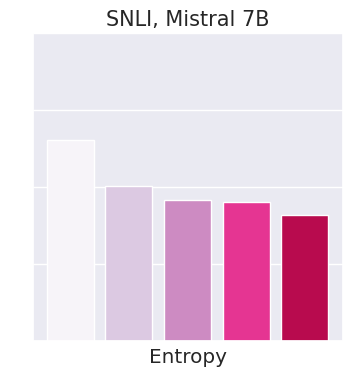
\includegraphics[height=3.6cm]{figures/appendix/entropy_acc_snli_7B}
        % \caption{}
    \end{subfigure}
    \begin{subfigure}[b]{0.23\textwidth}
        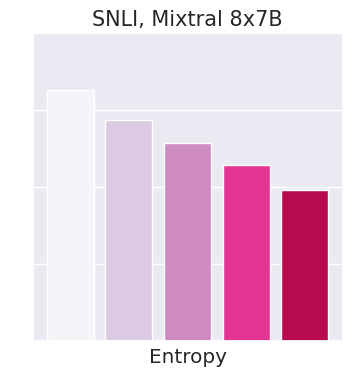
\includegraphics[height=3.6cm]{figures/appendix/entropy_acc_snli_8x7B}
        % \caption{}
    \end{subfigure}
    \begin{subfigure}[b]{0.23\textwidth}
        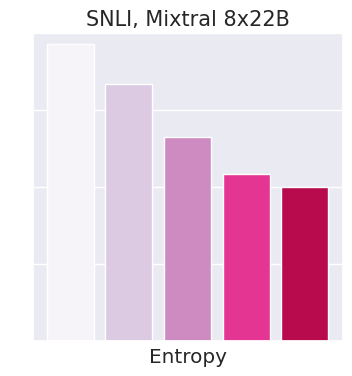
\includegraphics[height=3.6cm]{figures/appendix/entropy_acc_snli_8x22B}
        % \caption{}
    \end{subfigure}
    \caption{\textbf{Accuracy versus entropy.} We show how the accuracy of all other models changes as the entropy of the human label distributions increases.}
    \label{fig:entropy_accuracy_all}
\end{figure*}

\section{Prompt templates}

The prompt templates used for each task are presented in \cref{tab:prompt_template}.

\begin{table*}[t]
    \centering
    \small
    \begin{tabular}{lp{8cm}}
        \toprule
        \textbf{Benchmark} & \textbf{Prompt Template} \\
        \midrule
        MNLI, SNLI, ANLI & \begin{verbatim}

Premise: {{ x["premise"] }}
Hypothesis: {{ x["hypothesis"] }}
A. Entailment
B. Neutral
C. Contradiction
Answer: {{ x["answer"] }}


Premise: {{ premise }}
Hypothesis: {{ hypothesis }}
A. Entailment
B. Neutral
C. Contradiction
Answer: {{ choice_text }}
\end{verbatim} \\
\midrule
AbductiveNLI & \begin{verbatim}

Observation 1: {{ x["obs1"] }}
Observation 2: {{ x["obs2"] }}
A. {{ x["choices"]["A"] }}
B. {{ x["choices"]["B"] }}
Answer: {{ x["answer"] }}


Observation 1: {{ obs1 }}
Observation 2: {{ obs2 }}
A. {{ choices["A"] }}
B. {{ choices["B"] }}
Answer: {{ choice_text }}
\end{verbatim} \\
\midrule
HansNLI & \begin{verbatim}

Premise: {{ x["premise"] }}.
Hypothesis: {{ x["hypothesis"] }}.
A. Entailment
B. Non-Entailment
Answer: {{ x["answer"] }}


Premise: {{ premise }}.
Hypothesis: {{ hypothesis }}.
A. Entailment
B. Non-Entailment
Answer: {{ choice_text }}
\end{verbatim} \\
\bottomrule
\end{tabular}
\caption{Prompt Templates for each task}
\label{tab:prompt_template}
\end{table*}



\end{document}
